\documentclass[11pt,a4paper]{article}

\usepackage{float}
\usepackage{booktabs}
\usepackage{graphicx}
\usepackage{amsmath}
\usepackage{hyperref}
\renewcommand*\rmdefault{ppl}

\begin{document}

\begin{centering}{\underline{\Large{Experiment No. n}}}\\
\end{centering}

\section*{TITLE}
{\large PLACEHOLDER TITLE}

\section*{OBJECTIVES}

\begin{itemize}
	\item Objective uno
	\item Objective dos
	\item Objective tres
\end{itemize}

\section*{COMPONENTS REQUIRED}

\begin{itemize}
	\item Component uno
	\item Component dos
	\item Component tres
	\item Component cuatro
	\item Component cinco
	\item Component seis
\end{itemize}

\section*{THEORY}

\subsection*{Theoretical topic one}

\paragraph{}
bla bla bla\\
bla bla bla\\
bla bla bla\\
more of bla\\
bla bla bla\\


\paragraph{}
Some figure mysteriously appears!

\begin{figure}[h!]
	\centering
	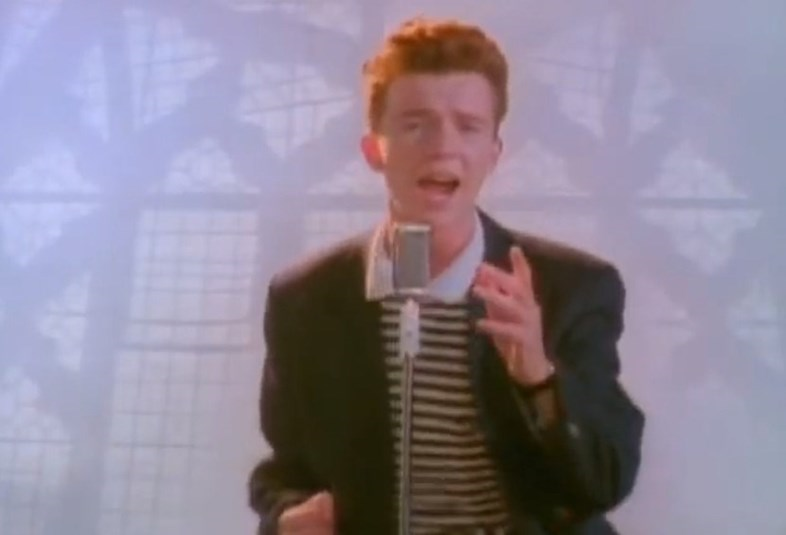
\includegraphics[width=450pt]{fig.png}
	\caption{A mysterious figure}
	\label{fig:fig1}
\end{figure}

\subsubsection*{Sub topic of theoretical topic}

\paragraph{}
stuff stuff stuff\\
stuff stuff stuff\\
stuff stuff stuff\\

\paragraph*{}
more of stuff\\
something significant?\\
nah more stuff\\
stuff stuff stuff\\

\section*{OBSERVATION}

\subsection*{Observation part one}

\subsubsection*{Circuit diagram maybe?}

\paragraph*{}
Description of what the circuit does.\\
A circuit incoming!\\

\begin{figure}[H]
	\centering
	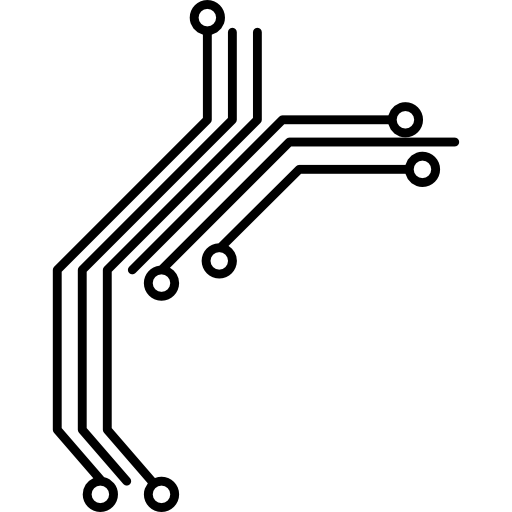
\includegraphics[width=150pt]{cir1.png}
	\caption{A circuit}
	\label{fig:circuit1}
\end{figure}

\subsection*{Observation part two}

\paragraph*{}
What we observed is that conducting observations make you very observant.\\
This is a very observable phenomenon and you gotta observe it.\\

\subsubsection*{Circuit diagram, again}

\begin{figure}[H]
	\centering
	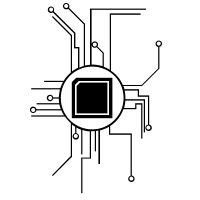
\includegraphics[width=150pt]{cir2.png}
	\caption{Yet another circuit diagram}
	\label{fig:circuit2}
\end{figure}


\subsection*{Final circuit}

\paragraph*{}
Finally we modified the circuit enough to reach to something nearing a conclusion.\\

\subsubsection*{Circuit diagram, last one seriously}

\begin{figure}[H]
	\centering
	
\includegraphics[width=150pt]{cir3.png}
	\caption{The last circuit}
	\label{fig:circuit3}
\end{figure}

\newpage

\section*{DISCUSSION AND CONCLUSION}

\paragraph{}
From this experiment, we got the knowledge of something we discussed earlier in the theory, evident in the objectives, extremely evident in the title. Now we claim that spending two and a half hours in the lab was very fruitful, not boring at all, we understood everything and a bit more, this could not have been done without the support of our teachers, I would like to thank my parents for this opportunity, also thanks to God and Prithvi Narayan Shah for bringing this country to existence and thanks especially to SJ sir for forcing us to do this before the 14th day.

\section*{REFERENCES}
\paragraph{}
\url{https://commons.wikimedia.org} % Get your images here.
\paragraph{}
other references here


\end{document}